
% Thank you Josh Davis for this template!
% https://github.com/jdavis/latex-homework-template/blob/master/homework.tex

\documentclass{article}

\newcommand{\hmwkTitle}{Final Report}

% % ----------

% Packages

\usepackage{fancyhdr}
\usepackage{extramarks}
\usepackage{amsmath}
\usepackage{amssymb}
\usepackage{amsthm}
\usepackage{amsfonts}
\usepackage{tikz}
\usepackage[plain]{algorithm}
\usepackage{algpseudocode}
\usepackage{enumitem}
\usepackage{chngcntr}

% Libraries

\usetikzlibrary{automata, positioning, arrows}

%
% Basic Document Settings
%

\topmargin=-0.45in
\evensidemargin=0in
\oddsidemargin=0in
\textwidth=6.5in
\textheight=9.0in
\headsep=0.25in

\linespread{1.1}

\pagestyle{fancy}
\lhead{\hmwkAuthorName}
\chead{}
\rhead{\hmwkClass\ (\hmwkClassInstructor): \hmwkTitle}
\lfoot{\lastxmark}
\cfoot{\thepage}

\renewcommand\headrulewidth{0.4pt}
\renewcommand\footrulewidth{0.4pt}

\setlength\parindent{0pt}
\setcounter{secnumdepth}{0}

\newcommand{\hmwkClass}{MATH 5345 / Regression Analysis}        % Class
\newcommand{\hmwkClassInstructor}{Dr. Sun}           % Instructor
\newcommand{\hmwkAuthorName}{\textbf{Joshua Mitchell}} % Author

%
% Title Page
%

\title{
    \vspace{2in}
    \textmd{\textbf{\hmwkClass:\ \hmwkTitle}}\\
    \normalsize\vspace{0.1in}\small\vspace{0.1in}\large{\textit{\hmwkClassInstructor}}
    \vspace{3in}
}

\author{\hmwkAuthorName}
\date{}

\renewcommand{\part}[1]{\textbf{\large Part \Alph{partCounter}}\stepcounter{partCounter}\\}

% Integral dx
\newcommand{\dx}{\mathrm{d}x}

%
% Various Helper Commands
%

% For derivatives
\newcommand{\deriv}[1]{\frac{\mathrm{d}}{\mathrm{d}x} (#1)}

% For partial derivatives
\newcommand{\pderiv}[2]{\frac{\partial}{\partial #1} (#2)}


% Alias for the Solution section header
\newcommand{\solution}{\textbf{\large Solution}}

% Formatting commands:

\newcommand{\mt}[1]{\ensuremath{#1}}
\newcommand{\nm}[1]{\textrm{#1}}

\newcommand\bsc[2][\DefaultOpt]{%
  \def\DefaultOpt{#2}%
  \section[#1]{#2}%
}
\newcommand\ssc[2][\DefaultOpt]{%
  \def\DefaultOpt{#2}%
  \subsection[#1]{#2}%
}
\newcommand{\bgpf}{\begin{proof} $ $\newline}

\newcommand{\bgeq}{\begin{equation*}}
\newcommand{\eeq}{\end{equation*}}	

\newcommand{\balist}{\begin{enumerate}[label=\alph*.]}
\newcommand{\elist}{\end{enumerate}}

\newcommand{\bilist}{\begin{enumerate}[label=\roman*)]}	

\newcommand{\bgsp}{\begin{split}}
% \newcommand{\esp}{\end{split}} % doesn't work for some reason.

\newcommand\prs[1]{~~~\textbf{(#1)}}

\newcommand{\lt}[1]{\textbf{Let: } #1}
     							   %  if you're setting it to be true
\newcommand{\supp}[1]{\textbf{Suppose: } #1}
     							   %  Suppose (if it'll end up false)
\newcommand{\wts}[1]{\textbf{Want to show: } #1}
     							   %  Want to show
\newcommand{\as}[1]{\textbf{Assume: } #1}
     							   %  if you think it follows from truth
\newcommand{\bpth}[1]{\textbf{(#1)}}

\newcommand{\step}[2]{\begin{equation}\tag{#2}#1\end{equation}}
\newcommand{\epf}{\end{proof}}

\newcommand{\dbs}[3]{\mt{#1_{#2_#3}}}

\newcommand{\sidenote}[1]{-----------------------------------------------------------------Side Note----------------------------------------------------------------
#1 \

---------------------------------------------------------------------------------------------------------------------------------------------}

% Analysis / Logical commands:

\newcommand{\br}{\mt{\mathbb{R}} }       % |R
\newcommand{\bq}{\mt{\mathbb{Q}} }       % |Q
\newcommand{\bn}{\mt{\mathbb{N}} }       % |N
\newcommand{\bc}{\mt{\mathbb{C}} }       % |C
\newcommand{\bz}{\mt{\mathbb{Z}} }       % |Z

\newcommand{\ep}{\mt{\epsilon} }         % epsilon
\newcommand{\fa}{\mt{\forall} }          % for all
\newcommand{\afa}{\mt{\alpha} }
\newcommand{\bta}{\mt{\beta} }
\newcommand{\mem}{\mt{\in} }
\newcommand{\exs}{\mt{\exists} }

\newcommand{\es}{\mt{\emptyset} }        % empty set
\newcommand{\sbs}{\mt{\subset} }         % subset of
\newcommand{\fs}[2]{\{\uw{#1}{1}, \uw{#1}{2}, ... \uw{#1}{#2}\}}

\newcommand{\lra}{ \mt{\longrightarrow} } % implies ----->
\newcommand{\rar}{ \mt{\Rightarrow} }     % implies -->

\newcommand{\lla}{ \mt{\longleftarrow} }  % implies <-----
\newcommand{\lar}{ \mt{\Leftarrow} }      % implies <--

\newcommand{\av}[1]{\mt{|}#1\mt{|}}  % absolute value

\newcommand{\prn}[1]{(#1)}
\newcommand{\bk}[1]{\{#1\}}

\newcommand{\ps}{\mt{\operatorname{+}} }
\newcommand{\ms}{\mt{\operatorname{-}} }

\newcommand{\ls}{\mt{\operatorname{<}} }
\newcommand{\gr}{\mt{\operatorname{>}} }

\newcommand{\lse}{\mt{\operatorname{\leq}} }
\newcommand{\gre}{\mt{\operatorname{\geq}} }

\newcommand{\eql}{ \mt{\operatorname{=}} }

\newcommand{\pr}{\mt{^\prime}} 		   % prime (i.e. R')
\newcommand{\uw}[2]{#1\mt{_{#2}}}
\newcommand{\uf}[2]{#1\mt{^{#2}}}
\newcommand{\frc}[2]{\mt{\frac{#1}{#2}}}
\newcommand{\lmti}[1]{\mt{\displaystyle{\lim_{#1 \to \infty}}}}
\newcommand{\limt}[2]{\mt{\displaystyle{\lim_{#1 \to #2}}}}

\newcommand{\bnm}[2]{\mt{#1\setminus{#2}}}
\newcommand{\bnt}[2]{\mt{\textrm{#1}\setminus{\textrm{#2}}}}
\newcommand{\bi}{\bnm{\mathbb{R}}{\mathbb{Q}}}

\newcommand{\urng}[2]{\mt{\bigcup_{#1}^{#2}}}
\newcommand{\nrng}[2]{\mt{\bigcap_{#1}^{#2}}}
\newcommand{\nck}[2]{\mt{{#1 \choose #2}}}

\newcommand{\nbho}[3]{\textrm{N(}#1, #2\textrm{) }\cap \textrm{ #3} \neq \emptyset}
     							   %  N(x, eps) intersect S \= emptyset
\newcommand{\nbhe}[3]{\textrm{N(}#1, #2\textrm{) }\cap \textrm{ #3} = \emptyset}
     							   %  N(x, eps) intersect S  = emptyset
\newcommand{\dnbho}[3]{\textrm{N*(}#1, #2\textrm{) }\cap \textrm{ #3} \neq \emptyset}
     							   %  N*(x, eps) intersect S \= emptyset
\newcommand{\dnbhe}[3]{\textrm{N*(}#1, #2\textrm{) }\cap \textrm{ #3} = \emptyset}
     							   %  N*(x, eps) intersect S = emptyset
     							   
\newcommand{\eqn}[1]{\[#1\]}
\newcommand{\splt}[1]{\begin{split}#1\end{split}}

\newcommand{\txt}[1]{\text{#1}} % Not new command, but remember \text for text in eqns
\newcommand{\tl}{\mt{\thicksim}}
\newcommand{\mn}[1]{\mt{\overline{#1}}}
\newcommand{\sg}{\mt{\sigma}}
\newcommand{\ssq}{\mt{\sigma^2}}	

\newcommand{\bh}[1]{\mathbf{\hat{\text{$#1$}}}}
\newcommand{\bth}{\mt{\bh{\beta}}}
\newcommand{\yh}{\mt{\bh{Y}}}

\newcommand{\exv}[1]{E[#1]}
\newcommand{\vrn}[1]{V[#1]}

\newcommand{\gv}{ \mt{|} }

\newcommand{\cov}[2]{\txt{Cov(#1, #2)}}

\newcommand{\img}[1]{
\begin{figure}[h]
  \includegraphics[width=0.5\linewidth]{#1}
\end{figure}
}
\newcommand\tab[1][1cm]{\hspace*{#1}}	
\newcommand{\sumin}[1]{\mt{\sum_{i = 1}^n #1}}		 
% ----------

% ----------

% Packages

\usepackage{fancyhdr}
\usepackage{extramarks}
\usepackage{amsmath}
\usepackage{amssymb}
\usepackage{amsthm}
\usepackage{amsfonts}
\usepackage{tikz}
\usepackage[plain]{algorithm}
\usepackage{algpseudocode}
\usepackage{enumitem}
\usepackage{chngcntr}
\usepackage{blkarray}

% Libraries

\usetikzlibrary{automata, positioning, arrows}

%
% Basic Document Settings
%

\topmargin=-0.45in
\evensidemargin=0in
\oddsidemargin=0in
\textwidth=6.5in
\textheight=9.0in
\headsep=0.25in

\linespread{1.1}

\pagestyle{fancy}
\lhead{\hmwkAuthorName}
\chead{}
\rhead{\hmwkClass\ (\hmwkClassInstructor): \hmwkTitle}
\lfoot{\lastxmark}
\cfoot{\thepage}

\renewcommand\headrulewidth{0.4pt}
\renewcommand\footrulewidth{0.4pt}

\setlength\parindent{0pt}
\setcounter{secnumdepth}{0}

\newcommand{\hmwkClass}{MATH 5345 / Regression Analysis}        % Class
\newcommand{\hmwkClassInstructor}{Dr. Sun}           % Instructor
\newcommand{\hmwkAuthorName}{\textbf{Gabriela Lara and Joshua Mitchell}} % Author

%
% Title Page
%

\title{
    \vspace{2in}
    \textmd{\textbf{\hmwkClass:\ \hmwkTitle}}\\
    \normalsize\vspace{0.1in}\small\vspace{0.1in}\large{\textit{\hmwkClassInstructor}}
    \vspace{3in}
}

\author{\hmwkAuthorName}
\date{}

\renewcommand{\part}[1]{\textbf{\large Part \Alph{partCounter}}\stepcounter{partCounter}\\}

% Integral dx
\newcommand{\dx}{\mathrm{d}x}

%
% Various Helper Commands
%

% For derivatives
\newcommand{\deriv}[1]{\frac{\mathrm{d}}{\mathrm{d}x} (#1)}

% For partial derivatives
\newcommand{\pderiv}[2]{\frac{\partial}{\partial #1} (#2)}


% Alias for the Solution section header
\newcommand{\solution}{\textbf{\large Solution}}

% Formatting commands:

\newcommand{\mt}[1]{\ensuremath{#1}}
\newcommand{\nm}[1]{\textrm{#1}}

\newcommand\bsc[2][\DefaultOpt]{%
  \def\DefaultOpt{#2}%
  \section[#1]{#2}%
}
\newcommand\ssc[2][\DefaultOpt]{%
  \def\DefaultOpt{#2}%
  \subsection[#1]{#2}%
}
\newcommand{\bgpf}{\begin{proof} $ $\newline}

\newcommand{\bgeq}{\begin{equation*}}
\newcommand{\eeq}{\end{equation*}}	

\newcommand{\balist}{\begin{enumerate}[label=\alph*.]}
\newcommand{\elist}{\end{enumerate}}

\newcommand{\bilist}{\begin{enumerate}[label=\roman*)]}	

\newcommand{\bgsp}{\begin{split}}
% \newcommand{\esp}{\end{split}} % doesn't work for some reason.

\newcommand\prs[1]{~~~\textbf{(#1)}}

\newcommand{\lt}[1]{\textbf{Let: } #1}
     							   %  if you're setting it to be true
\newcommand{\supp}[1]{\textbf{Suppose: } #1}
     							   %  Suppose (if it'll end up false)
\newcommand{\wts}[1]{\textbf{Want to show: } #1}
     							   %  Want to show
\newcommand{\as}[1]{\textbf{Assume: } #1}
     							   %  if you think it follows from truth
\newcommand{\bpth}[1]{\textbf{(#1)}}

\newcommand{\step}[2]{\begin{equation}\tag{#2}#1\end{equation}}
\newcommand{\epf}{\end{proof}}

\newcommand{\dbs}[3]{\mt{#1_{#2_#3}}}

\newcommand{\sidenote}[1]{-----------------------------------------------------------------Side Note----------------------------------------------------------------
#1 \

---------------------------------------------------------------------------------------------------------------------------------------------}

% Analysis / Logical commands:

\newcommand{\br}{\mt{\mathbb{R}} }       % |R
\newcommand{\bq}{\mt{\mathbb{Q}} }       % |Q
\newcommand{\bn}{\mt{\mathbb{N}} }       % |N
\newcommand{\bc}{\mt{\mathbb{C}} }       % |C
\newcommand{\bz}{\mt{\mathbb{Z}} }       % |Z

\newcommand{\ep}{\mt{\epsilon} }         % epsilon
\newcommand{\fa}{\mt{\forall} }          % for all
\newcommand{\afa}{\mt{\alpha} }
\newcommand{\bta}{\mt{\beta} }
\newcommand{\mem}{\mt{\in} }
\newcommand{\exs}{\mt{\exists} }

\newcommand{\es}{\mt{\emptyset} }        % empty set
\newcommand{\sbs}{\mt{\subset} }         % subset of
\newcommand{\fs}[2]{\{\uw{#1}{1}, \uw{#1}{2}, ... \uw{#1}{#2}\}}

\newcommand{\lra}{ \mt{\longrightarrow} } % implies ----->
\newcommand{\rar}{ \mt{\Rightarrow} }     % implies -->

\newcommand{\lla}{ \mt{\longleftarrow} }  % implies <-----
\newcommand{\lar}{ \mt{\Leftarrow} }      % implies <--

\newcommand{\av}[1]{\mt{|}#1\mt{|}}  % absolute value

\newcommand{\prn}[1]{(#1)}
\newcommand{\bk}[1]{\{#1\}}

\newcommand{\ps}{\mt{\operatorname{+}} }
\newcommand{\ms}{\mt{\operatorname{-}} }

\newcommand{\ls}{\mt{\operatorname{<}} }
\newcommand{\gr}{\mt{\operatorname{>}} }

\newcommand{\lse}{\mt{\operatorname{\leq}} }
\newcommand{\gre}{\mt{\operatorname{\geq}} }

\newcommand{\eql}{ \mt{\operatorname{=}} }

\newcommand{\pr}{\mt{^\prime}} 		   % prime (i.e. R')
\newcommand{\uw}[2]{#1\mt{_{#2}}}
\newcommand{\uf}[2]{#1\mt{^{#2}}}
\newcommand{\frc}[2]{\mt{\frac{#1}{#2}}}
\newcommand{\lmti}[1]{\mt{\displaystyle{\lim_{#1 \to \infty}}}}
\newcommand{\limt}[2]{\mt{\displaystyle{\lim_{#1 \to #2}}}}

\newcommand{\bnm}[2]{\mt{#1\setminus{#2}}}
\newcommand{\bnt}[2]{\mt{\textrm{#1}\setminus{\textrm{#2}}}}
\newcommand{\bi}{\bnm{\mathbb{R}}{\mathbb{Q}}}

\newcommand{\urng}[2]{\mt{\bigcup_{#1}^{#2}}}
\newcommand{\nrng}[2]{\mt{\bigcap_{#1}^{#2}}}
\newcommand{\nck}[2]{\mt{{#1 \choose #2}}}

\newcommand{\nbho}[3]{\textrm{N(}#1, #2\textrm{) }\cap \textrm{ #3} \neq \emptyset}
     							   %  N(x, eps) intersect S \= emptyset
\newcommand{\nbhe}[3]{\textrm{N(}#1, #2\textrm{) }\cap \textrm{ #3} = \emptyset}
     							   %  N(x, eps) intersect S  = emptyset
\newcommand{\dnbho}[3]{\textrm{N*(}#1, #2\textrm{) }\cap \textrm{ #3} \neq \emptyset}
     							   %  N*(x, eps) intersect S \= emptyset
\newcommand{\dnbhe}[3]{\textrm{N*(}#1, #2\textrm{) }\cap \textrm{ #3} = \emptyset}
     							   %  N*(x, eps) intersect S = emptyset
     							   
\newcommand{\eqn}[1]{\[#1\]}
\newcommand{\splt}[1]{\begin{split}#1\end{split}}

\newcommand{\txt}[1]{\text{#1}} % Not new command, but remember \text for text in eqns
\newcommand{\tl}{\mt{\thicksim} }
\newcommand{\mn}[1]{\mt{\overline{#1}}}
\newcommand{\sg}{\mt{\sigma}}
\newcommand{\ssq}{\mt{\sigma^2}}	

\newcommand{\bh}[1]{\mathbf{\hat{\text{$#1$}}}}
\newcommand{\bth}{\mt{\bh{\beta}}}
\newcommand{\yh}{\mt{\bh{Y}}}

\newcommand{\exv}[1]{\txt{E[}#1\txt{]}}
\newcommand{\vrn}[1]{V[#1]}

\newcommand{\gv}{ \mt{|} }

\newcommand{\cov}[2]{\txt{Cov(#1, #2)}}

\newcommand{\img}[1]{
\begin{figure}[h]
  \includegraphics[width=0.5\linewidth]{#1}
\end{figure}
}
\newcommand{\simg}[1]{
  \includegraphics[width=0.35\linewidth]{#1}
}
\newcommand{\wimg}[1]{
\begin{figure}[h]
  \includegraphics[width=1\linewidth]{#1}
\end{figure}
}
\newcommand\tab[1][1cm]{\hspace*{#1}}	
\newcommand{\sumin}[1]{\mt{\sum_{i = 1}^n #1}}	

\newcommand{\brm}[1]{\begin{pmatrix} #1 \end{pmatrix}}

\newcommand{\inm}[1]{\mt{\left\[ \begin{smallmatrix} #1 \end{smallmatrix} \right\]}}

\newcommand{\lbm}[4]{
	  \begin{blockarray}{#1} % a c for every row, plus the c-labels
        #2 \\ % & c-label1 & c-label2 & c-label3...
      \begin{block}{c(#3)} % a c for every column only
        #4 % r-label1 & data & data & data ... \\
           % r-label2 & data & data & data ... \\
           % ...
           % r-labeln & data & data & data ... \\
      \end{block}
    \end{blockarray}
}

% Example:
% \[\lbm{ccccc}{& H & y & d}{cccc}{H & 4 & 4 & 4 \\
% Y & 3 & 3 & 3 \\
% D & 2 & 2 & 2 \\
% D & 2 & 2 & 2 \\}\]

\newcommand{\unds}[2]{\mt{\underset{#1}{#2}}} % stuff underneath!	 
% ----------

\begin{document}

\maketitle

\newpage

\tableofcontents

\listoftables

\listoffigures

\newpage

\section{Abstract}

  A multiple linear regression was calculated to predict the gas mileage of a car (its MPG) based on the number of cylinders, displacement, horsepower, weight, acceleration, model year, and origin of the car. The initial model had problems with non-constant variance and multicollinearity. A transformation on the response variable and an additional interaction regressor was added to improve the homoscedasticity and the explanatory power of the model, resulting in an \uf{R}{2} value of 0.89. Only a subset of the seven regressors and an interaction term turned out to be significant.

\newpage

\section{Introduction}

  The Auto MPG data set, from the UC Irvine Machine Learning Repository, contains 397 samples of various models of vehicles. The goal of the analysis is to learn to predict a vehicle's gas mileage (mpg) given other attributes of the vehicle (e.g. its weight, model year, origin, etc).
  
  The data contains a total of nine attributes. Three are discrete (origin, model year, and number of cylinders), one is alphanumeric (model name), and the rest are continuous. The model name column was thrown out, and model year and number of cylinders were interpreted as continuous variables.
  
  The data also had some missing values (6), but they constituted a negligible amount of the data, so they were removed.
  
\newpage

\section{Discussion of Models and Analysis Results}

\subsection{Original Full Model Analysis}

\textbf{Original Full Model:}

\textbf{mpg (c) \tl wgt (c) + modelyr (mvd) + origin (mvd) + hp (c) + displ (c) + cylnum (mvd) + acc (c)}

\begin{table}[ht]
\centering
\begin{tabular}{rrrrrr}
  \hline
 & Estimate & Std. Error & t value & Pr($>$$|$t$|$) & Significance \\ 
  \hline
(Intercept) & -18.3106 & 4.6933 & -3.90 & 0.0001 & *** \\ 
  wgt\_c & -0.0067 & 0.0007 & -10.23 & 0.0000 & ***  \\ 
  modelyr\_mvd & 0.7805 & 0.0519 & 15.03 & 0.0000 & ***  \\ 
  origin\_mvd2 & 2.6340 & 0.5665 & 4.65 & 0.0000 & ***  \\ 
  origin\_mvd3 & 2.8557 & 0.5528 & 5.17 & 0.0000 & ***  \\ 
  hp\_c & -0.0174 & 0.0137 & -1.27 & 0.2056 & \\ 
  displ\_c & 0.0241 & 0.0077 & 3.14 & 0.0018 & ** \\ 
  cylnum\_mvd & -0.5123 & 0.3222 & -1.59 & 0.1126 & \\ 
  acc\_c & 0.0845 & 0.0984 & 0.86 & 0.3913 & \\ 
   \hline
\end{tabular}
\caption{R Summary of original full model (relating mpg to the rest)}
\label{tab:myfirsttable}
\end{table}


\begin{table}[ht]
\centering
\begin{tabular}{lrrrrrr}
  \hline
 & Df & Sum Sq & Mean Sq & F value & Pr($>$F) & Significance\\ 
  \hline
wgt\_c & 1 & 16470.05 & 16470.05 & 1505.92 & 0.0000 & ***  \\ 
  modelyr\_mvd & 1 & 2756.94 & 2756.94 & 252.08 & 0.0000 & ***  \\ 
  origin\_mvd & 2 & 261.23 & 130.61 & 11.94 & 0.0000 & ***  \\ 
  hp\_c & 1 & 8.96 & 8.96 & 0.82 & 0.3659 & \\ 
  displ\_c & 1 & 77.03 & 77.03 & 7.04 & 0.0083 & ** \\ 
  cylnum\_mvd & 1 & 29.10 & 29.10 & 2.66 & 0.1037 & \\ 
  acc\_c & 1 & 8.06 & 8.06 & 0.74 & 0.3913 &  \\ 
  Residuals & 382 & 4177.89 & 10.94 &  & & \\ 
   \hline
\end{tabular}
\caption{R ANOVA of original full model (relating mpg to the rest)}
\label{tab:myfirsttable}
\end{table}


\begin{table}[ht]
\centering
\begin{tabular}{rrrr}
  \hline
 & GVIF & Df & GVIF\verb|^|(1/(2*Df)) \\ 
  \hline
wgt\_c & 11.07 & 1.00 & 3.33 \\ 
  modelyr\_mvd & 1.30 & 1.00 & 1.14 \\ 
  origin\_mvd & 2.09 & 2.00 & 1.20 \\ 
  hp\_c & 9.98 & 1.00 & 3.16 \\ 
  displ\_c & 22.87 & 1.00 & 4.78 \\ 
  cylnum\_mvd & 10.74 & 1.00 & 3.28 \\ 
  acc\_c & 2.62 & 1.00 & 1.62 \\ 
   \hline
\end{tabular}
\caption{VIF of each regressor in the Full Original Model}
\label{tab:fulloriginalvif}
\end{table}

\clearpage
\newpage 

\begin{figure}
	\centering
	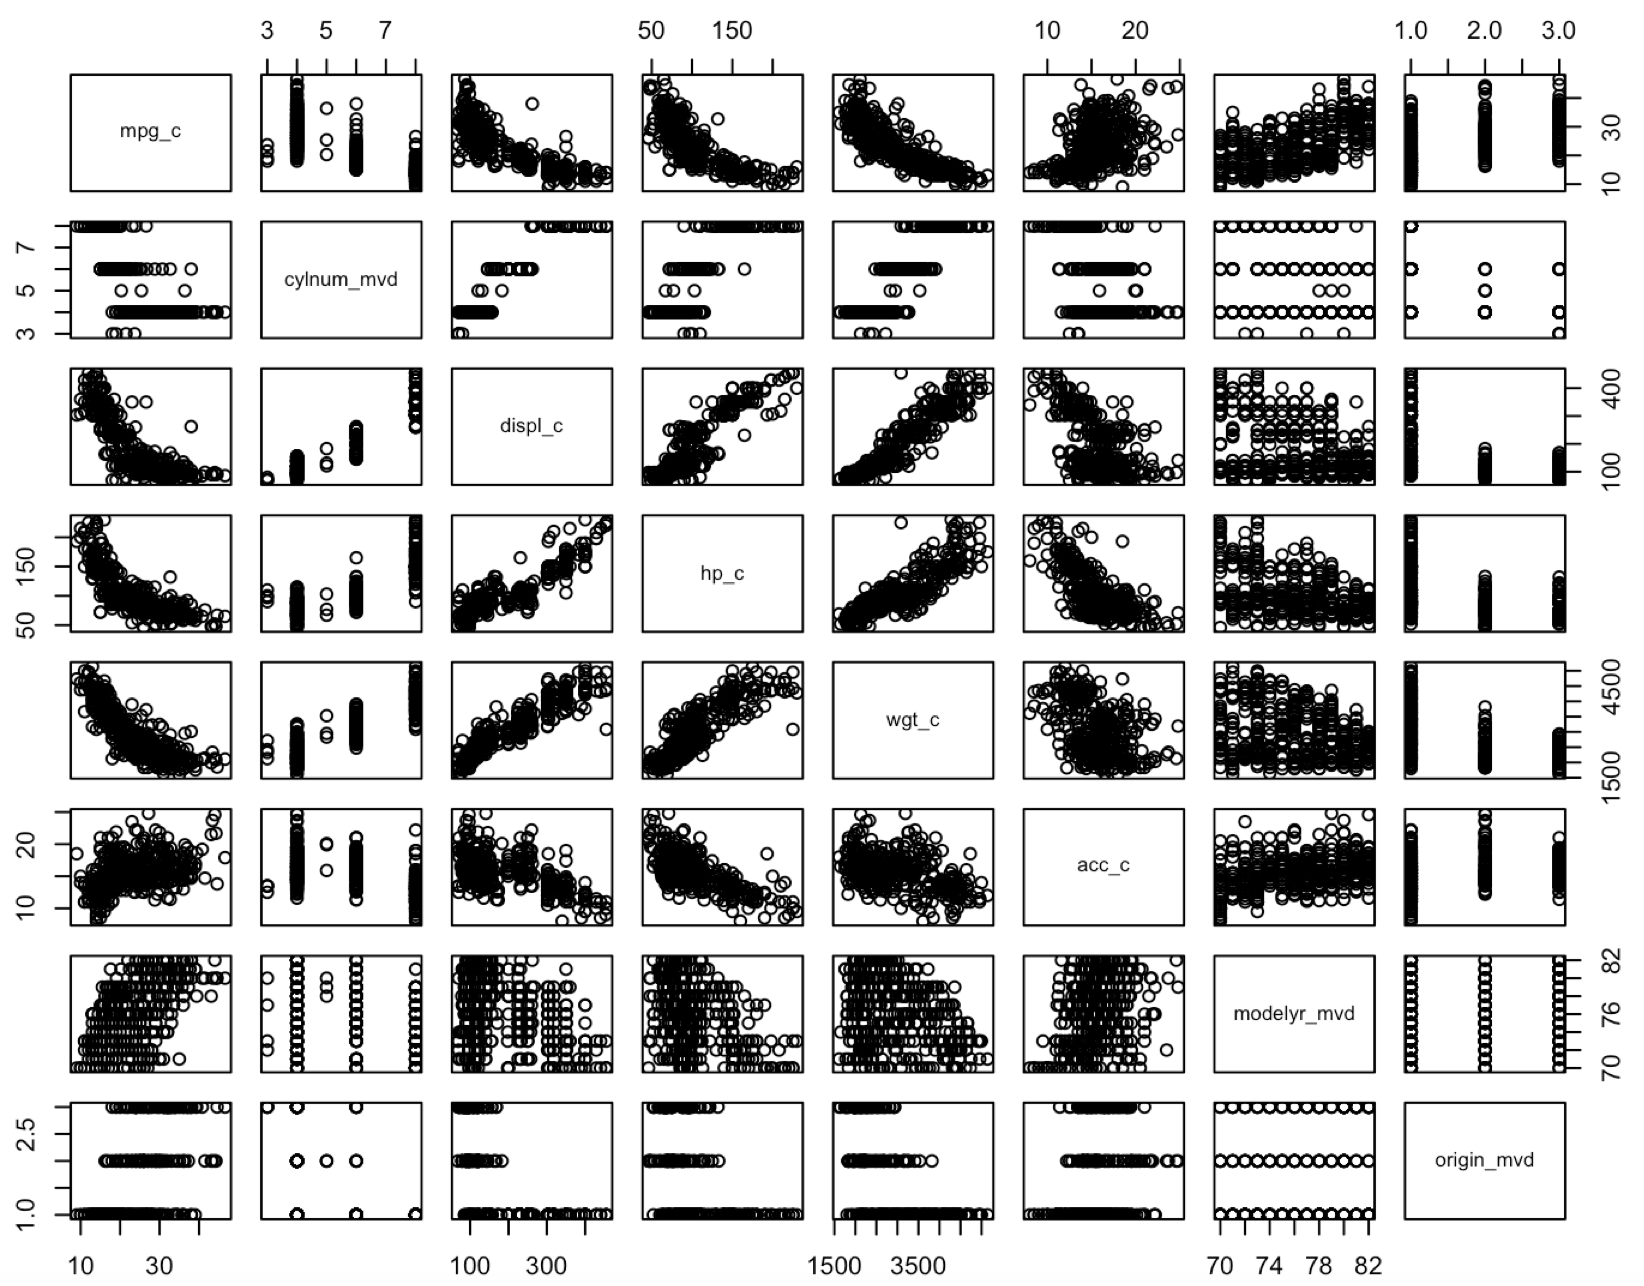
\includegraphics[width=1\linewidth]{1p_ScPlMtr}
	\caption[Scatterplot Matrix of the Original Full Model]
	{A scatterplot matrix between all the variables in the automobile data set}
\end{figure}

\clearpage
\newpage 

\begin{figure}
	\centering
	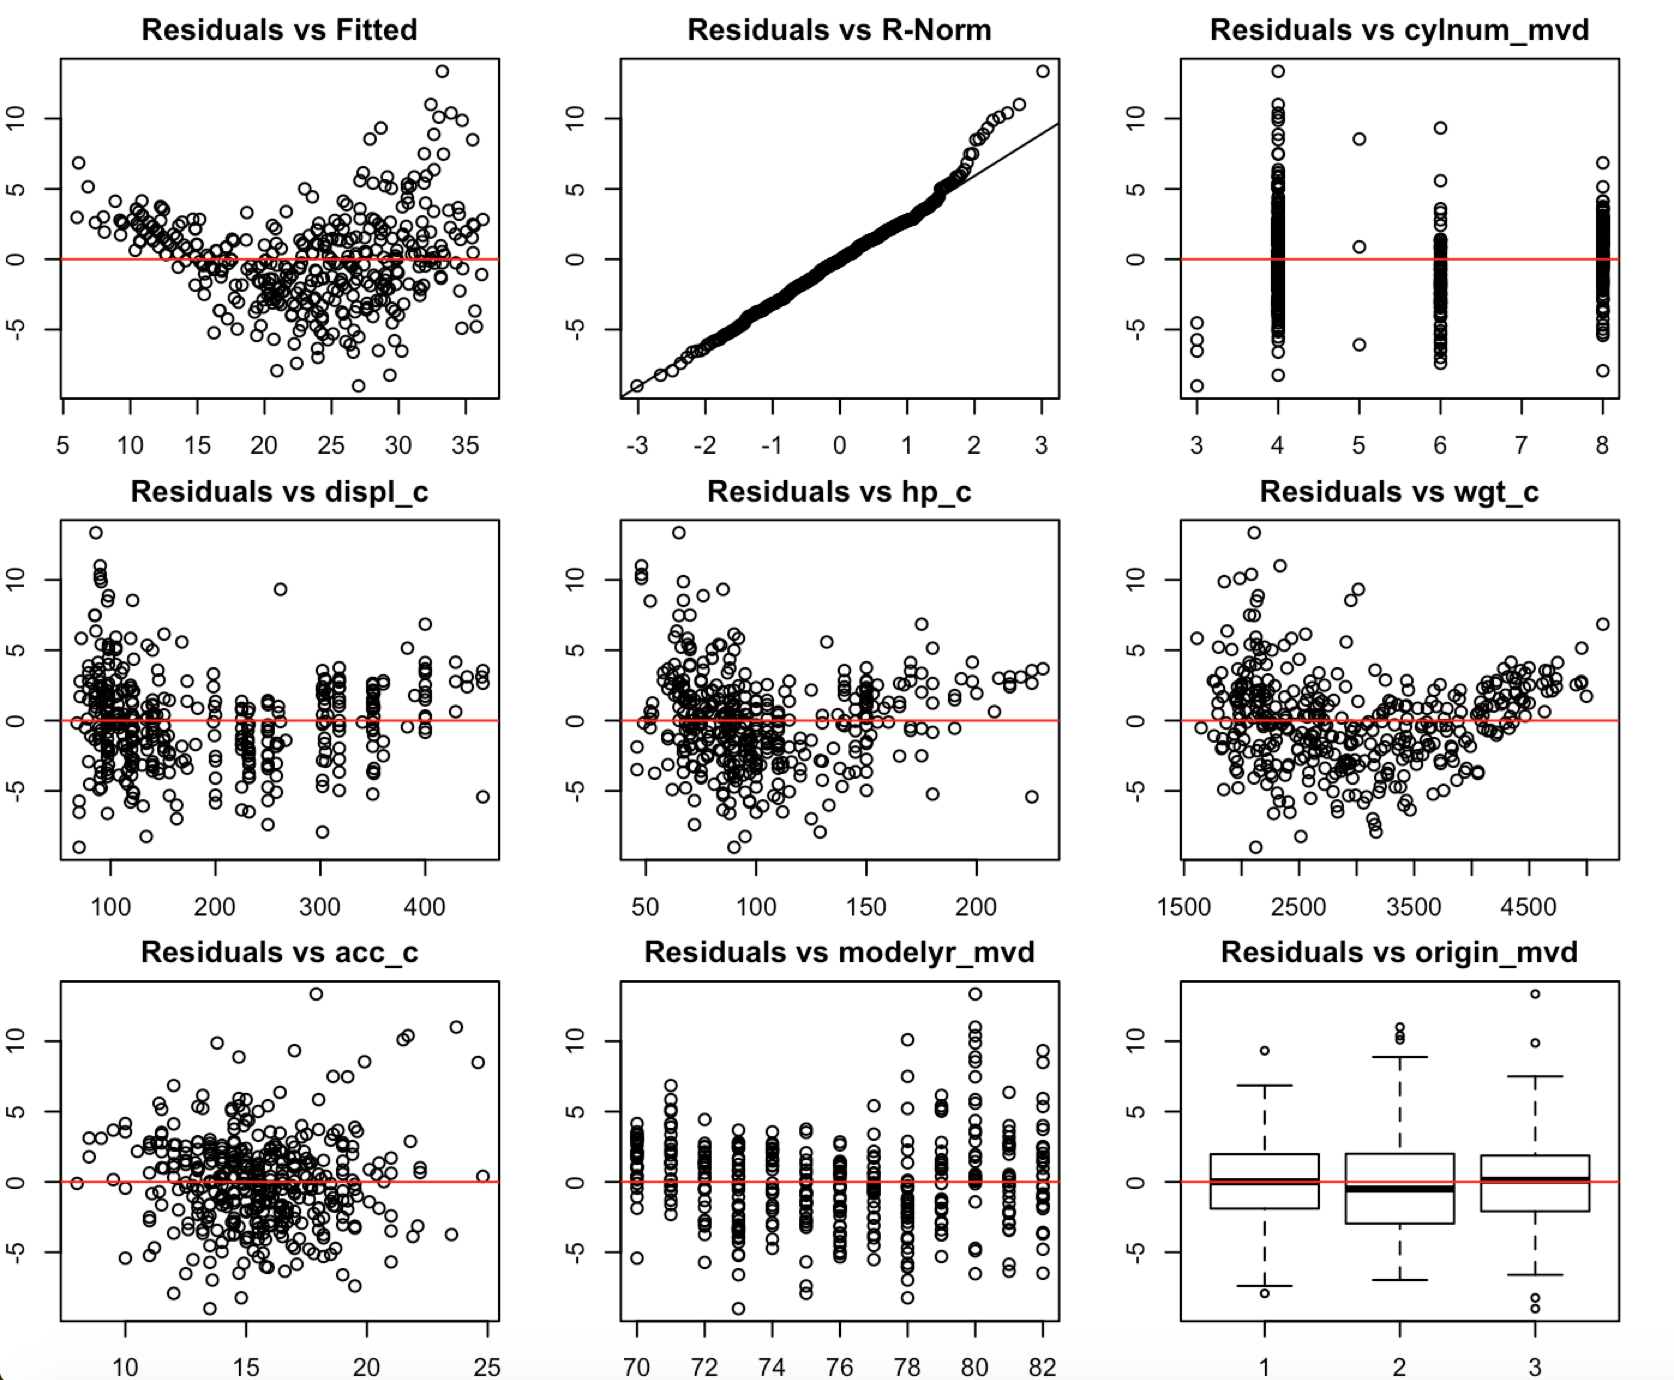
\includegraphics[width=1\linewidth]{2-10p_resall}
	\caption[Residual Plots of the Original Full Model]
	{A Residual vs Fitted, a Residual vs R-Norm, and Residual vs Regressors plots of the Original Full Model}
\end{figure}

\clearpage
\newpage 

\begin{table}[ht]
\centering
\begin{tabular}{rlrrl}
  \hline
 & Regressor & F\_Statistic & P\_Value & Significance \\ 
  \hline
1 & Displacement & 9.89 & 0.00 & ** \\ 
  2 & Weight & 104.63 & 0.00 & *** \\ 
  3 & HP & 1.61 & 0.21 & none \\ 
  4 & Cylinder Num & 2.53 & 0.11 & none \\ 
   \hline
\end{tabular}
\caption{A partial F test on each of the regressors with high VIF scores}
\label{tab:partialfhighvif}
\end{table}

\begin{figure}
	\centering
	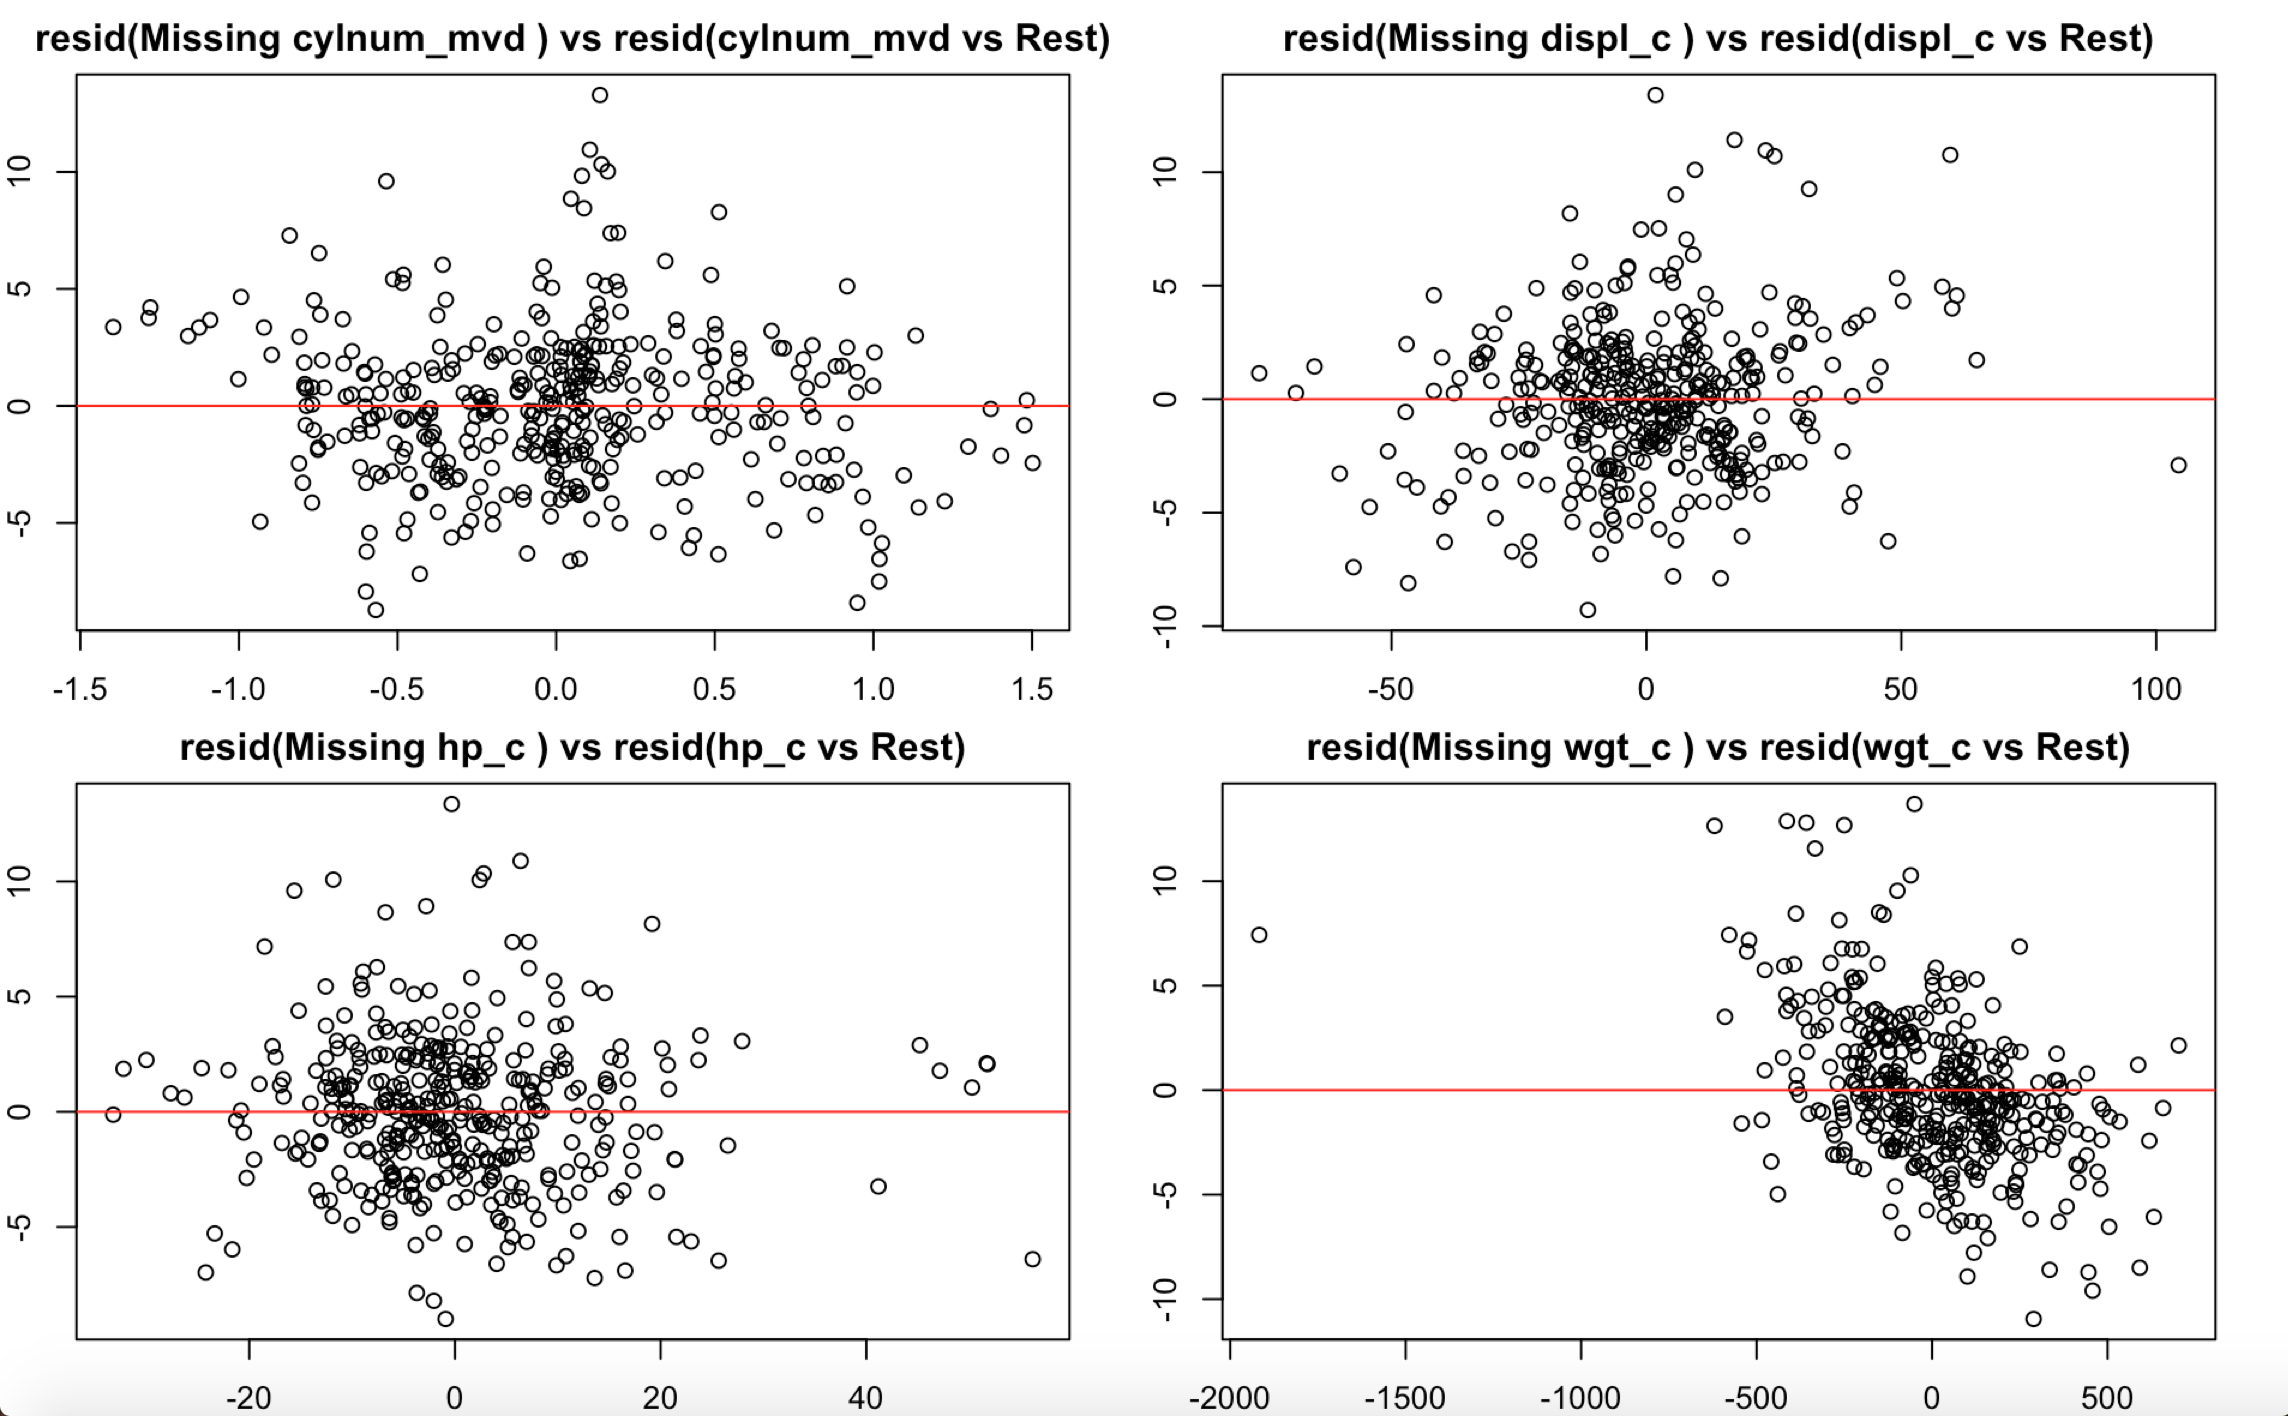
\includegraphics[width=1\linewidth]{11-14p_PrRgall4}
	\caption[Partial regression plots on high VIF regressors]
	{Partial regression plots on each of the regressors with high VIF scores}
\end{figure}

\clearpage
\newpage

A full multiple linear regression was fitted on the data set with mileage (mpg) as the response variable and number of cylinders (cylnum), displacement (displ), horsepower (hp), weight (wgt), acceleration (acc), model year (modelyr), and origin (origin) as the predictor variables. The following five key assumptions were examined:

\balist
\item Normality of errors: Based on figure 2, it appears that the residuals are mostly normally distributed with a light tail.
\item Independence of errors: Based on figure 2, our errors might be nontrivially dependent due to the quadratic shape of the Residuals vs Fitted plot.
\item Constant variance of errors: Based on figure 2's Residuals vs Fitted plot, it appears that, due to the inconsistency of the spread of the residuals, constant variance is not upheld.
\item An expected error value of 0: Based on figure 2's Residuals vs Fitted plot, it is likely that this is upheld (due to half the data being roughly above 0 and the other half being below).
\item Linearity: Based on the significance of multiple coefficient estimates for each regressor in Table 1, it appears that our response variable is linearly related to our predictor variables. However, in the scatterplot (Figure 1), some regressors have a linear relationship with the response variable and some don't. In the Residuals vs Fitted plot (Figure 2), it takes a somewhat quadratic shape, but both ways can be argued. There is a gray area, but overall, linearity can be argued for.
\elist

Correlation among variables was also examined. Figure 1 and Table 3 indicate a strong relationship between hp, wgt, displ, and cylnum. Further inspection was done with partial regression plots and a partial f test for each of said variables. At this point, due to the significance of some variables and lack of significance of others from the partial f tests, it was concluded that a log transformation should be done on the response variable (mpg), due to the quadratic pattern in the Residual vs Fitted plot, and possibly an addition of an interaction term.


\clearpage 
\newpage

\subsection{Transformed Full Model Analysis}

\textbf{Transformed Full Model:}

\textbf{log(mpg) (c) \tl wgt (c) + modelyr (mvd) + origin (mvd) + hp (c) + displ (c) + cylnum (mvd) + acc (c)}

\begin{figure}[h]
	\centering
	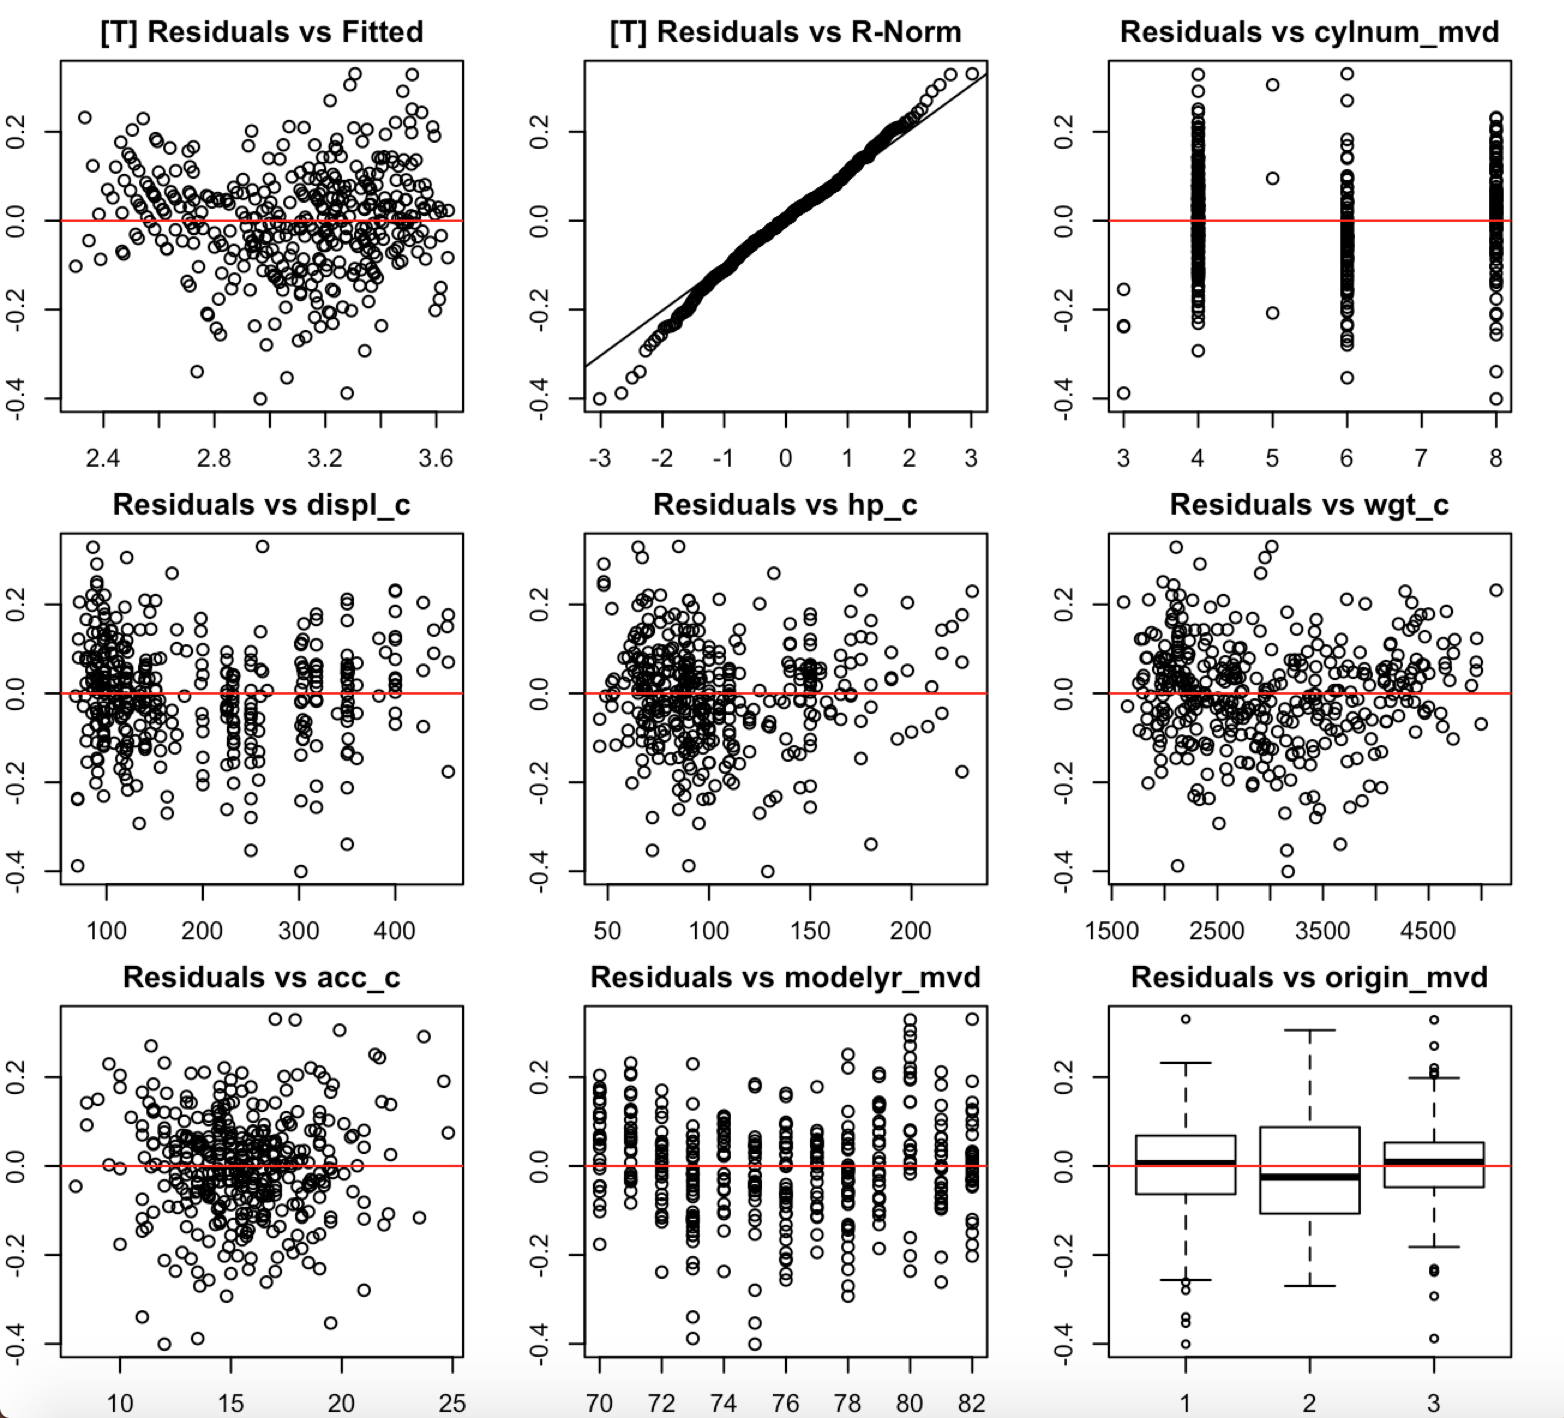
\includegraphics[width=0.95\linewidth]{15-23t_resall}
	\caption[Residual Plots of the Transformed Full Model]
	{A Residual vs Fitted, a Residual vs R-Norm, and Residual vs Regressors plots of the Transformed Full Model}
\end{figure}

\clearpage
\newpage

\begin{table}[ht]
\centering
\begin{tabular}{rlrrl}
  \hline
 & Regressor & F\_Statistic & P\_Value & Significance \\ 
  \hline
1 & Displacement & 8.39 & 0.00 & ** \\ 
  2 & Weight & 126.68 & 0.00 & *** \\ 
  3 & HP & 9.10 & 0.00 & ** \\ 
  4 & Cylinder Num & 6.35 & 0.01 & * \\ 
   \hline
\end{tabular}
\caption{A partial F test on each of the regressors with high VIF scores on the Transformed Full Model}
\label{tab:partialfhighvif}
\end{table}

\begin{figure}
	\centering
	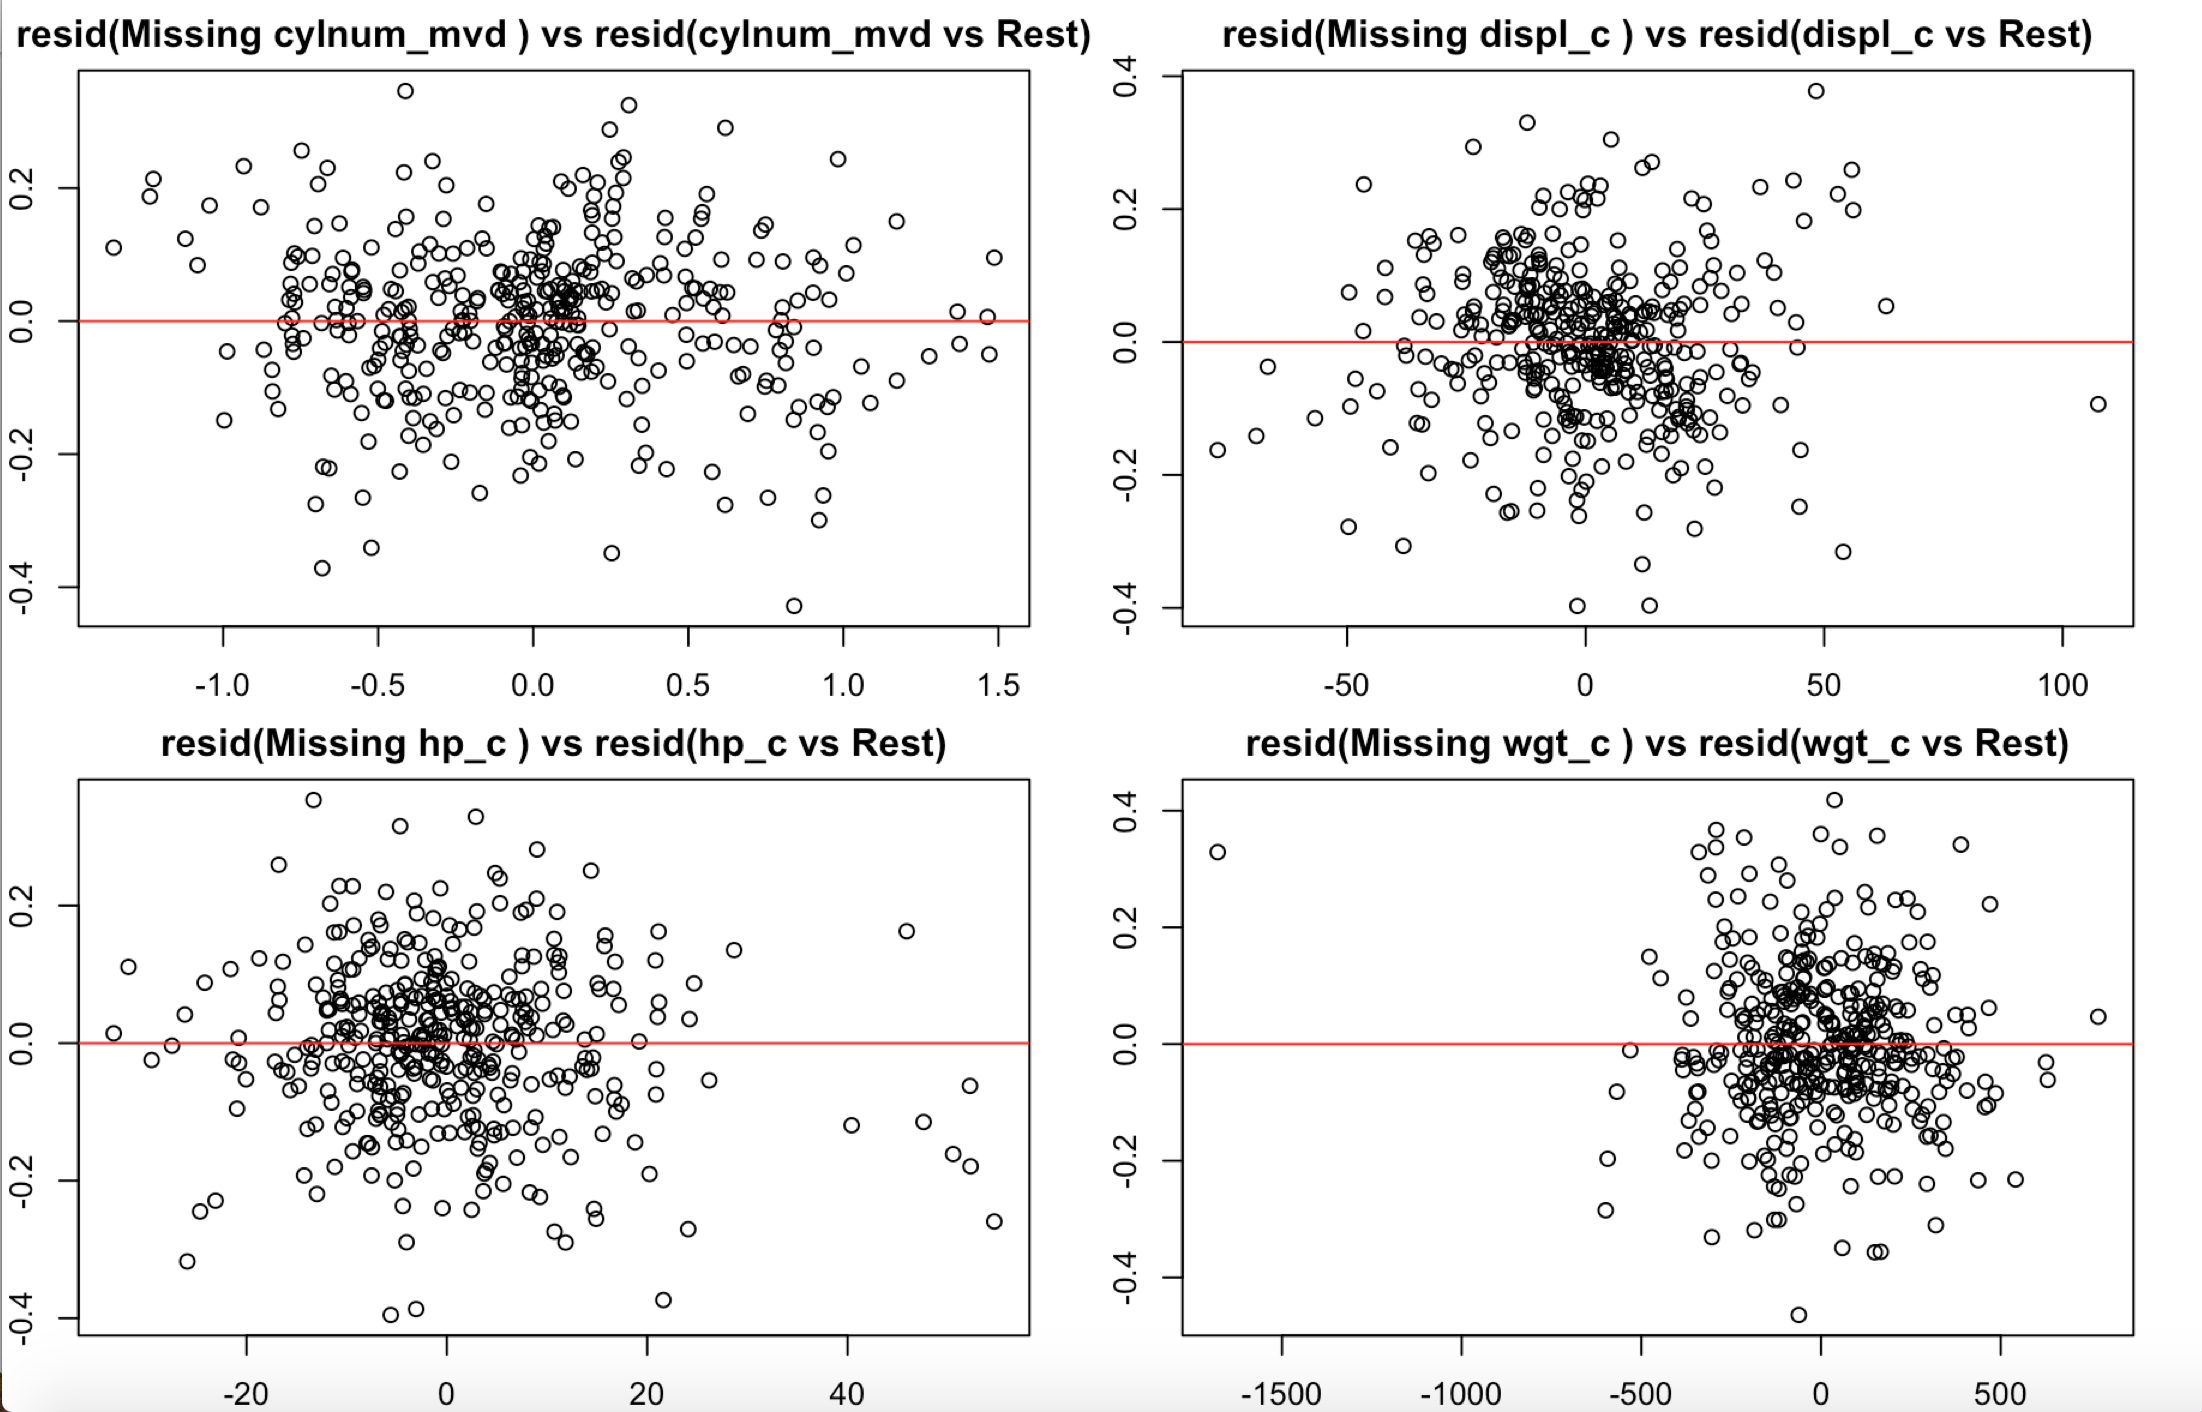
\includegraphics[width=1\linewidth]{24-27t_PrRgall4}
	\caption[Partial regression plots on high VIF regressors on the Transformed Full Model]
	{Partial regression plots on each of the regressors with high VIF scores on the Transformed Full Model}
\end{figure}

\clearpage
\newpage

A new model was created with a log transformation on the response variable and then examined. Fortunately, the transformation dampened the quadratic pattern (increasing the independence of the errors) and stabilized the variance of the residuals.

\

However, the partial regression plots and partial f tests were redone with the same 4 regressors with mixed results. The transformation made the insignificant regressors (hp and cylnum) more significant (**, and *, respectively), however, the partial regression plots showed that the explanatory power of these two regressors was not significant.

\clearpage
\newpage

\subsection{Interaction Terms Analysis}

\begin{table}[ht]
\centering
\begin{tabular}{rlrrr}
  \hline
 & Model & R\_Sq & AR\_Sq & MS\_res \\ 
  \hline
1 & Interaction & 0.88 & 0.87 & 7.90 \\ 
  2 & Transformed + Interaction & 0.90 & 0.90 & 0.01 \\ 
   \hline
\end{tabular}
\caption{A chart comparing the Untransformed Full Model with all combinations of interaction terms for the high VIF regressors against the same model with a log transformation on the response variable (mpg)}
\label{tab:myfirsttable}
\end{table}

It was suspected, due to the somewhat significant difference between the partial f tests and partial regression plots of the transformed full model, that there was possible multicollinearity, so it was decided that an interaction term should be added. Due to the number of possible interaction terms, it was decided that all regressors plus all possible combinations of the regressors with high VIFs should be modeled and then compared to the original full model. The addition of these interaction terms resulted in a significant increase in \uf{R}{2}. A plain full model with these interaction terms was also compared to a transformed full model with the same interaction terms, and it was concluded that, given that interaction terms were going to be included, the transformed model was better based on its \uf{R}{2}. In the next section, other model metrics will be considered.

\newpage

\subsection{Model Selection Analysis}

\begin{table}[ht]
\centering
\begin{tabular}{rlrrrr}
  \hline
 & Selection\_Method & Num\_Regressors & R\_Sq & Adj\_R\_Sq & MS\_res \\ 
  \hline
1 & Forward & 6.00 & 0.89 & 0.89 & 0.01 \\ 
  2 & Backward & 16.00 & 0.90 & 0.90 & 0.01 \\ 
  3 & Stepwise & 6.00 & 0.89 & 0.89 & 0.01 \\ 
   \hline
\end{tabular}
\caption{Statistics about the models outputted from Forward, Backward, and Stepwise Selection algorithms in R (note that the model selected by Forward and Stepwise selection is identical, so just the Forward model will be considered in further sections)}
\label{tab:selectionalgorithmmodelcomparison}
\end{table}

\begin{table}[ht]
\centering
\begin{tabular}{rrrr}
  \hline
 & GVIF & Df & GVIF\verb|^|(1/(2*Df)) \\ 
  \hline
wgt\_c & 13.83 & 1.00 & 3.72 \\ 
  modelyr\_mvd & 1.27 & 1.00 & 1.13 \\ 
  origin\_mvd & 1.74 & 2.00 & 1.15 \\ 
  hp\_c & 37.47 & 1.00 & 6.12 \\ 
  acc\_c & 2.61 & 1.00 & 1.62 \\ 
  wgt\_c:hp\_c & 58.06 & 1.00 & 7.62 \\ 
   \hline
\end{tabular}
\caption{VIF of each regressor in the Forward Model}
\label{tab:forwardmodelvif}
\end{table}

\begin{table}[ht]
\centering
\begin{tabular}{rrrr}
  \hline
 & GVIF & Df & GVIF\verb|^|(1/(2*Df)) \\ 
  \hline
wgt\_c & 3110.02 & 1.00 & 55.77 \\ 
  modelyr\_mvd & 1.44 & 1.00 & 1.20 \\ 
  origin\_mvd & 3.01 & 2.00 & 1.32 \\ 
  hp\_c & 2806.06 & 1.00 & 52.97 \\ 
  displ\_c & 10568.29 & 1.00 & 102.80 \\ 
  cylnum\_mvd & 975.92 & 1.00 & 31.24 \\ 
  acc\_c & 3.64 & 1.00 & 1.91 \\ 
  wgt\_c:hp\_c & 27058.36 & 1.00 & 164.49 \\ 
  hp\_c:displ\_c & 39680.75 & 1.00 & 199.20 \\ 
  wgt\_c:displ\_c & 11724.72 & 1.00 & 108.28 \\ 
  wgt\_c:cylnum\_mvd & 9069.37 & 1.00 & 95.23 \\ 
  hp\_c:cylnum\_mvd & 9125.25 & 1.00 & 95.53 \\ 
  displ\_c:cylnum\_mvd & 19861.83 & 1.00 & 140.93 \\ 
  wgt\_c:hp\_c:cylnum\_mvd & 41867.56 & 1.00 & 204.62 \\ 
  wgt\_c:displ\_c:cylnum\_mvd & 15077.88 & 1.00 & 122.79 \\ 
  hp\_c:displ\_c:cylnum\_mvd & 44842.29 & 1.00 & 211.76 \\ 
   \hline
\end{tabular}
\caption{VIF of each regressor in the Backward Model}
\label{tab:backwardmodelvif}
\end{table}

\clearpage
\newpage 

\begin{figure}
	\centering
	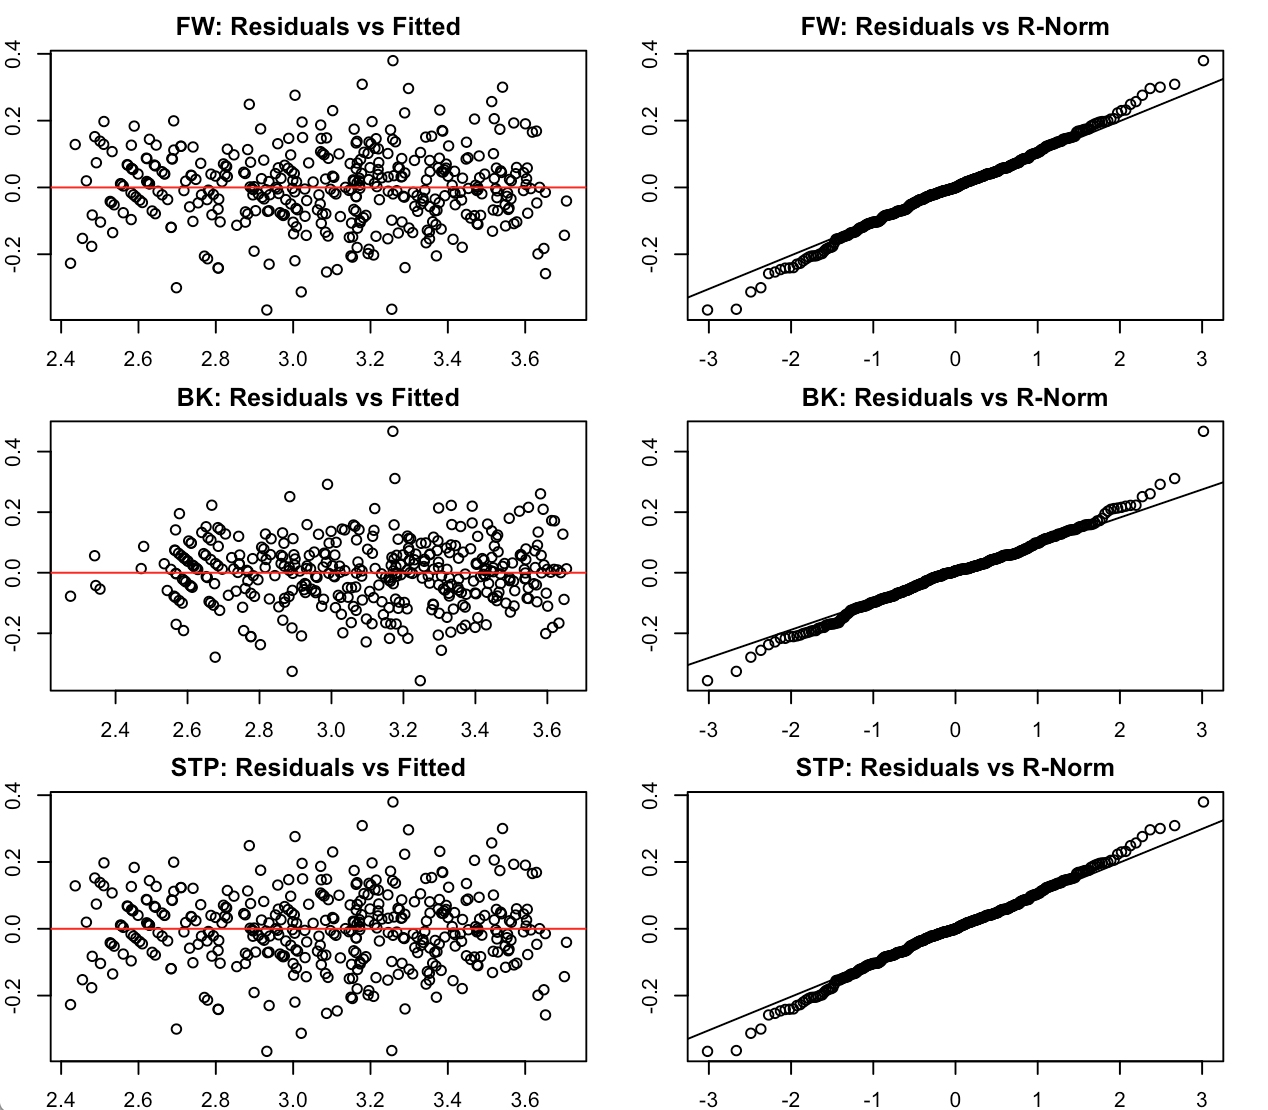
\includegraphics[width=1\linewidth]{28ti_resfittednorm}
	\caption[Residuals vs Fitted and vs Random Normal plots for Forward, Backward, and Stepwise Models]
	{Residuals vs Fitted and vs Random Normal plots for Forward, Backward, and Stepwise Models}
\end{figure}

\clearpage
\newpage 

In order to select the most significant variables, several tests were applied: Forward, Backwards and Stepwise (Table 7).

\

The Forward and Stepwise selection algorithms both selected a model with 6 variables (5 original variables and 1 interaction term). The Backwards selection algorithm selected a model with 16 variables (mostly interaction terms).

\

The Backward selection model has a slightly higher \uf{R}{2}, but with slightly less degrees of freedom (due to the increased parameters) and possibly more complexity.

\

The VIF values of each regressor of each model were also examined. As expected, the VIF for the known correlated variables was still high, but, more importantly, the other variables showed little correlation.

\

The 5 key assumptions for each model were also checked (see Figure 6) and no major problems were observed. Outliers and influential points are examined in the next section.

\clearpage
\newpage 

\subsection{Influential Points Analysis}

\begin{table}[ht]
\centering
\begin{tabular}{rlrlr}
  \hline
 & Model & Num\_Infl\_Pnts & Percent\_Infl\_Pnts & Common\_Infl\_Pnts \\ 
  \hline
1 & Forward & 20.00 & 5.12\% & 14.00 \\ 
  2 & Backward & 36.00 & 9.21\% & 14.00 \\ 
   \hline
\end{tabular}
\caption{Influential point comparison of Forward Model vs Backward Model}
\label{tab:myfirsttable}
\end{table}

\begin{table}[ht]
\centering
\begin{tabular}{rlrrr}
  \hline
 & Model & R\_Sq & AR\_Sq & MS\_res \\ 
  \hline
1 & Forward w/o Infl & 0.91 & 0.91 & 0.01 \\ 
  2 & Backward w/o Infl & 0.90 & 0.90 & 0.01 \\ 
   \hline
\end{tabular}
\caption{Forward Model with no influential points vs Backward Model with no influential points}
\label{tab:forwardvsbackwardnoinfluential}
\end{table}

It was observed that the Backward model had almost twice as many points deemed influential as the Forward model, indicating that the Forward model might be either more resilient to influential points or a better model of the data in general, since both models have a roughly equal \uf{R}{2} and \uw{MS}{residuals}.

\clearpage
\newpage

\subsection{Final Model Choice}

\textbf{log(mpg) (c) \tl modelyr (mvd) + origin (mvd) + hp (c) + acc (c) + wgt (c) * hp (c)}

\begin{table}[ht]
\centering
\begin{tabular}{rrrrrr}
  \hline
 & Estimate & Std. Error & t value & Pr($>$$|$t$|$) & Significance\\ 
  \hline
(Intercept) & 2.1373 & 0.1735 & 12.32 & 0.00001 & *** \\ 
  wgt\_c & -0.0004 & 0.0000 & -14.76 & 0.00001 & *** \\ 
  modelyr\_mvd & 0.0309 & 0.0018 & 17.59 & 0.00001 & *** \\ 
  origin\_mvd2 & 0.0558 & 0.0177 & 3.14 & 0.00180 & ** \\ 
  origin\_mvd3 & 0.0455 & 0.0180 & 2.52 & 0.01210 & * \\ 
  hp\_c & -0.0064 & 0.0009 & -7.06 & 0.00001 & *** \\ 
  acc\_c & -0.0053 & 0.0034 & -1.59 & 0.11180 & \\ 
  wgt\_c:hp\_c & 0.0000013 & 0.0000002 & 6.71 & 0.00001 & *** \\ 
   \hline
\end{tabular}
\caption{R Summary of the final model}
\label{tab:summaryfinalmodel}
\end{table}

\begin{table}[ht]
\centering
\begin{tabular}{lrrrrrr}
  \hline
 & Df & Sum Sq & Mean Sq & F value & Pr($>$F) & Significance \\ 
  \hline
wgt\_c & 1 & 34.62 & 34.62 & 2714.64 & 0.0000 & *** \\ 
  modelyr\_mvd & 1 & 4.72 & 4.72 & 369.94 & 0.0000 & *** \\ 
  origin\_mvd & 2 & 0.25 & 0.12 & 9.78 & 0.0001 & *** \\ 
  hp\_c & 1 & 0.11 & 0.11 & 8.87 & 0.0031 & ** \\ 
  acc\_c & 1 & 0.001 & 0.00 & 0.26 & 0.6078 & \\ 
  wgt\_c:hp\_c & 1 & 0.57 & 0.57 & 45.04 & 0.0000 & *** \\ 
  Residuals & 383 & 4.88 & 0.01 &  &  & \\ 
   \hline
\end{tabular}
\caption{R ANOVA of the final model}
\label{tab:anovafinalmodel}
\end{table}

Many model combinations were considered, but the simplicity, high \uf{R}{2}, low \uw{MS}{residuals}, and resilience to influential points of the Forward model made it the number one choice. Tables 12 and 13 indicate the R Summary and R ANOVA of the chosen model.

\newpage

\section{Conclusion}

A model that mostly satisfies the 5 key assumptions of multiple linear regression and also explains 89\% of the variance in the response variable (mpg) was found, which, by most metrics is a good job. It does appear that there is a significant linear relationship between the gas mileage of a car and other attributes like its weight and model year.

\

The initial model appeared to violate 2 of the 5 key assumptions (independent errors and constant variance of residuals) and seemed to have some multicollinearity problems among regressors. A log transformation on the response variable eased the 2 key assumption violations (as well as increased the predictive ability of the model), and the addition of an interaction term compensated for the correlation of two of the variables (as well as increased the predictive ability of the model. Since the models generated by the selection algorithms had similar predictive power, the one that had the least influential points was chosen.

\newpage

\section{References}

The data was acquired from UC Irvine's Machine Learning Repository at the following web address:

https://archive.ics.uci.edu/ml/datasets/auto+mpg

\end{document}